% ---------------------------------------------------------------------
% --- Arquivo principal e os demais serao os dos capitulos.
% --- EXPRESSÔES ENTRE <> DEVERÂO SER COMPLETADAS COM A INFORMAÇÂO ESPECÌFICA DO TRABALHO 
% ---------------------------------------------------------------------
\documentclass[ruledheader]{abnt_UFF}[abntex2]
\usepackage[alf]{abntex2cite}

%--- pacotes para hiphenizacao e acentuacao em portugues
\usepackage[brazil]{babel}
%\usepackage[latin1]{inputenc}
\usepackage[utf8]{inputenc}
\usepackage[T1]{fontenc}

%--- pacote para figuras
\usepackage{epsf}
\usepackage[dvips]{epsfig,graphicx}
\usepackage{subfigure}

%--- pacote de simbolos
\usepackage{latexsym}
\usepackage{textcomp}

%--- simbolos matematicos
\usepackage{amsmath}
\usepackage{amssymb}

%--- pacote para gerar pseudo-codigo
\usepackage{algorithm}
\usepackage{algorithmic}
\floatname{algorithm}{Algoritmo}

%--- outros pacotes
\usepackage{url}
\usepackage{longtable}
\usepackage{pdflscape}
\usepackage{setspace}
\usepackage{booktabs}
\usepackage{alltt}
\usepackage[flushleft]{threeparttable}
\renewcommand{\ttdefault}{txtt}

%Tabela Colorida
\usepackage{colortbl}
\usepackage{multicol}
\usepackage{multirow}
\usepackage{rotating}
\usepackage{caption}

\hyphenation{
    a-de-qua-da-men-te
    di-men-sio-na-men-to
}

%---------usando tipo de fonte padrao
\renewcommand{\ABNTchapterfont}{\bfseries\fontfamily{cmr}\fontseries{b}\selectfont}
\renewcommand{\ABNTsectionfont}{\bfseries\fontfamily{cmr}}

% --- -----------------------------------------------------------------
% --- Documento Principal.
% --- -----------------------------------------------------------------
% \usepackage[pdftex]{hyperref}
% \hypersetup{colorlinks, sitecolor=black, pdftex}

\begin{document}
    % --- Para elementos em português, remover.
    \renewcommand{\listfigurename}{Lista de Figuras}
    \renewcommand{\figurename}{Figura}
    \renewcommand{\listtablename}{Lista de Tabelas}
    \renewcommand{\tablename}{Tabela}
    \renewcommand{\contentsname}{Sumário}
    \renewcommand{\refname}{Referências}
    \renewcommand{\appendixname}{Apêndices}
    \renewcommand{\chaptername}{Capítulo}

% --- -----------------------------------------------------------------
% --- Titulo, abstract, dedicatorias e agradecimentos.
% --- Indice geral, lista de figuras e tabelas.
% --- -----------------------------------------------------------------
    	% --- -----------------------------------------------------------------
	% --- Elementos usados na Capa e na Folha de Rosto.
	% --- EXPRESS�ES ENTRE <> DEVER�O SER COMPLETADAS COM A INFORMA��O ESPEC�FICA DO TRABALHO
	% --- E OS S�MBOLOS <> DEVEM SER RETIRADOS 
	% --- -----------------------------------------------------------------
	\cleardoublepage
	\thispagestyle{empty}
	
	\vspace{-60mm}
	  \begin{singlespace}
	    \begin{center}
	      {\large UNIVERSIDADE FEDERAL DO ACRE}
	      \vskip4.0cm{\textbf{\Large Gustavo Moreira Oliveira de Castro}}
	      \vskip5.0cm {\textbf{Análise comparativa de estimadores monoculares de profundidade relativa}}
	    \end{center}
	    \begin{center}
	      \vskip10.0cm{\textbf{RIO BRANCO\\2024}}
	    \end{center}
	  \end{singlespace}
	% --- -----------------------------------------------------------------
	% --- Folha de rosto. (Obrigatorio)
	% --- ----------------------------------------------------------------
	\cleardoublepage
	\thispagestyle{empty}
	
	\vspace{-60mm}
	  \begin{center}
	    {\large UNIVERSIDADE FEDERAL DO ACRE}\\
	    \vspace{3cm}
	    {\large Gustavo Moreira Oliveira de Castro} \\
	    \vspace{3cm}
	    
	    {\large Análise comparativa de estimadores monoculares de profundidade relativa} \\
	    \vspace{1.5cm}
	  \end{center}
	
	\noindent
	  \begin{flushright}
	    \begin{minipage}[t]{8cm}
	     \textcolor{black}{Proposta de dissertação de mestrado submetida ao Programa de Pós-Graduação em Ciência da Computação na Universidade Federal do Acre como requisito parcial para obtenção do título de mestre em Ciência da Computação. Linha de Pesquisa: Sistemas Computacionais Inteligentes}
	    \end{minipage}
	  \end{flushright}
	
	\vskip1.50cm
	  \begin{center}
	    \small Orientador: \\
	    Prof. Dr. {Roger Fredy Larico Chavez}\vskip3.5cm 
	  \end{center}
	  \begin{center}
	    \vspace{4mm}
	    RIO BRANCO \\
	    %\vspace{6mm}
	    2024
	  \end{center}
	
	\thispagestyle{empty}
	% --- -----------------------------------------------------------------
	% --- Termo de aprovacao. (Obrigatorio)
	% --- ----------------------------------------------------------------
	\cleardoublepage
	\thispagestyle{empty}
	
	\vspace{-60mm}
	
	\begin{center}
	  {\large Gustavo Moreira Oliveira de Castro} \\
	  \vspace{7mm}
	
	  {\large Análise comparativa de estimadores monoculares de profundidade relativa} \\
	  \vspace{10mm}
	\end{center}
	
	\noindent
	\begin{flushright}
	  \begin{minipage}[t]{8cm}
	
		\textcolor{black}{Proposta de dissertação de mestrado submetida ao Programa de Pós-Graduação em Ciência da Computação na Universidade Federal do Acre como requisito parcial para obtenção do título de mestre em Ciência da Computação. Linha de Pesquisa: Sistemas Computacionais Inteligentes}.
	
	  \end{minipage}
	\end{flushright}
	
	\vspace{1.0 cm}
	\noindent
	
	Approved in <MONTH> of <YEAR>. \\
	\begin{flushright}
	  \parbox{11cm}
	  {
	    \begin{center}
	      \vspace{3mm}
	      \rule{11cm}{.1mm} \\
	      Prof. Dr. Roger Fredy Larico Chavez (Presidente, Orientador)\\
	      Universidade Federal do Acre
	      \vspace{3mm}
	    \end{center}
     
     \begin{center}
	      \vspace{3mm}
	      \rule{11cm}{.1mm} \\
	      Prof. Dra. Ana Beatriz Alvarez Mamani (Co-orientadora)\\
	      Universidade Federal do Acre
	      \vspace{3mm}
	    \end{center}
     
     \begin{center}
	      \vspace{3mm}
	      \rule{11cm}{.1mm} \\
	      Prof. Dr. ...\\
	      Universidade Federal do Acre
	      \vspace{3mm}
	    \end{center}
	  }
	\end{flushright}
	
	\begin{center}
	  \vspace{4mm}
	  RIO BRANCO \\
	  %\vspace{6mm}
	  2024
	\end{center}
	
	% --- -----------------------------------------------------------------
	% --- Dedicatoria.(Opcional)
	% --- ----------------------------------------------------------------
	\cleardoublepage
	\thispagestyle{empty}
	\vspace*{200mm}
	
	\begin{flushright}
	  {\em
	dfsaas
	    \\
	   - 
	    \\ 
	    
	  }
	\end{flushright}
	\newpage
	
	% --- -----------------------------------------------------------------
	% --- Agradecimentos.(Opcional)
	% --- ----------------------------------------------------------------
	\pretextualchapter{Agradecimentos}
	\hspace{5mm}
	
	...
	
	% --- -----------------------------------------------------------------
	% --- Resumo em portugues.(Obrigatorio)
	% --- ----------------------------------------------------------------
	\begin{resumo}
	
	  \begin{center}{
	    \textbf{Análise comparativa de estimadores monoculares de profundidade relativa}}
	  \end{center}
	
	\begin{spacing}{1.0}
		Informação de profundidade possui grande importância em diversas aplicações que exigem informação geométrica, como veículos autônomos, navegação robótica, realidade aumentada e geração de conteúdo por inteligência artificial. Mapas de profundidade podem ser adquiridos com sensores ou através de estimação por métodos passivos. O desenvolvimento de técnicas de aprendizado profundo propiciou a viabilidade da tarefa de estimação monocular de profundidade, em que é utilizada uma única imagem RGB como entrada de um sistema de rede neural. O presente trabalho se propõe a realizar uma análise comparativa dos estimadores monoculares do estado da arte em termos de métricas presentes na literatura, transferência de domínio de relativo para métrico e o emprego em aplicações práticas. Os resultados preliminares demonstraram o funcionamento do método de transformação de intensidades para transferência de domínio, no entanto, ajustes ainda precisam ser feitos no algoritmo para tratamento de funções geradas que não são monotônicas.
	\end{spacing}
	{\hspace{-8mm} \bf{Palavras-chave}}: Mapa de profundidade; Aprendizado Profundo; Detecção de Objetos 3D; Estimação Monocular de Profundidade.
	
	\end{resumo}
	
	% --- -----------------------------------------------------------------
	% --- Resumo em lingua estrangeira.(Obrigatorio)
	% --- ----------------------------------------------------------------
	\begin{abstract}
	
		Depth information has great importance in various applications that require geometric information, such as autonomous vehicles, robotic navigation, augmented reality, and artificial intelligence content generation. Depth maps can be acquired with sensors or through estimation by passive methods. The development of deep learning techniques has made monocular depth estimation a feasible task, where a single RGB image is used as input to a neural network system. This work aims to perform a comparative analysis of state-of-the-art monocular depth estimators in terms of metrics found in the literature, domain transfer from relative to metric, and application in practical scenarios. Preliminary results have demonstrated the effectiveness of the intensity transform method for domain transfer, however, adjustments still need to be made to the algorithm to address generated functions that are not monotonic.
	
	{\hspace{-8mm} \bf{Keywords}}: Depth Map; Deep Learning; 3D Object Detection; Monocular Depth Estimation.
	
	\end{abstract}
	
	% --- -----------------------------------------------------------------
	% --- Lista de figuras.(Opcional)
	% --- -----------------------------------------------------------------
	%\cleardoublepage
	\listoffigures
	
	% --- -----------------------------------------------------------------
	% --- Lista de tabelas.(Opcional)
	% --- -----------------------------------------------------------------
	\cleardoublepage
	%\label{pag:last_page_introduction}
	\listoftables
	\cleardoublepage
	
	% --- -----------------------------------------------------------------
	% --- Sumario.(Obrigatorio)
	% --- -----------------------------------------------------------------
	\pagestyle{ruledheader}
	\tableofcontents
	
% --- -----------------------------------------------------------------
% --- Insercao dos capitulos.
% --- -----------------------------------------------------------------
    \pagestyle{ruledheader}
    \setcounter{page}{1}
    \pagenumbering{arabic}
    
\chapter{Introdução}

\section{Contextualização}

Informação de profundidade é uma das representações mais úteis para o entendimento de ambientes físicos \cite{lasinger2019towards} \cite{zhou2019does}. São também uma parte importante da caracterização de relações geométricas de uma determinada cena. As imagens de profundidades (ou mapas de profundidade) desempenham um papel importante em uma série de aplicações que envolvem visão computacional \cite{eigen2014depth}.  Entre elas, podemos citar: compreensão de cenas \cite{jaritz2018sparse}, veículos autônomos \cite{song2021self}, navegação de robôs \cite{ma2019sparse} navegação de VANTs, \cite{padhy2023monocular} fazendas inteligentes \cite{farkhani2019sparse}, e realidade aumentada \cite{du2020depthlab}. 

% \textit{Simultaneos Localization and Mapping} (SLAM) \cite{hu2012robust}

Os mapas de profundidade representam as distâncias de cada ponto (ou pixel) numa cena física em relação ao eixo do dispositivo de captura. Podem ser representados por imagens em escala de cinza, com as cores dos pixels sendo proporcionais à distância, com cinzas mais claros para objetos mais próximos e tons mais escuros para pontos mais afastados (e vice-versa) \cite{dourado2020multi}.

% \begin{figure}[h]
%     \centering
%     \includegraphics[width=\textwidth]{fig/example_depth.png}
%     \caption{Exemplo de mapa de profundidade do \textit{dataset Nyu Depth V2}. No primeiro quadro, a imagem RGB, no segundo, o mapa de profundidade em escala de cinza, no terceiro uma colorização artificial para o mapa de profundidade.}
%     \label{dmap}
% \end{figure}


Para capturar tais imagens geralmente são empregadas câmeras RGB-D, que podem prover tanto informação de profundidade quanto imagens coloridas da cena. Entre suas tecnologias mais comuns, são encontrados diversos tipos de aquisição que podem ser baseados em visão estereoscópica, que trabalha com múltiplos ângulos de visão, sensores \textit{Time-of-Flight} (ToF) que emprega projeção de lasers infravermelhos (IR) estruturados e técnicas mais precisas como o LiDAR (\textit{Light Detection and Ranging}) \cite{castellano2023performance}.




% \begin{figure}
%     \centering   
%     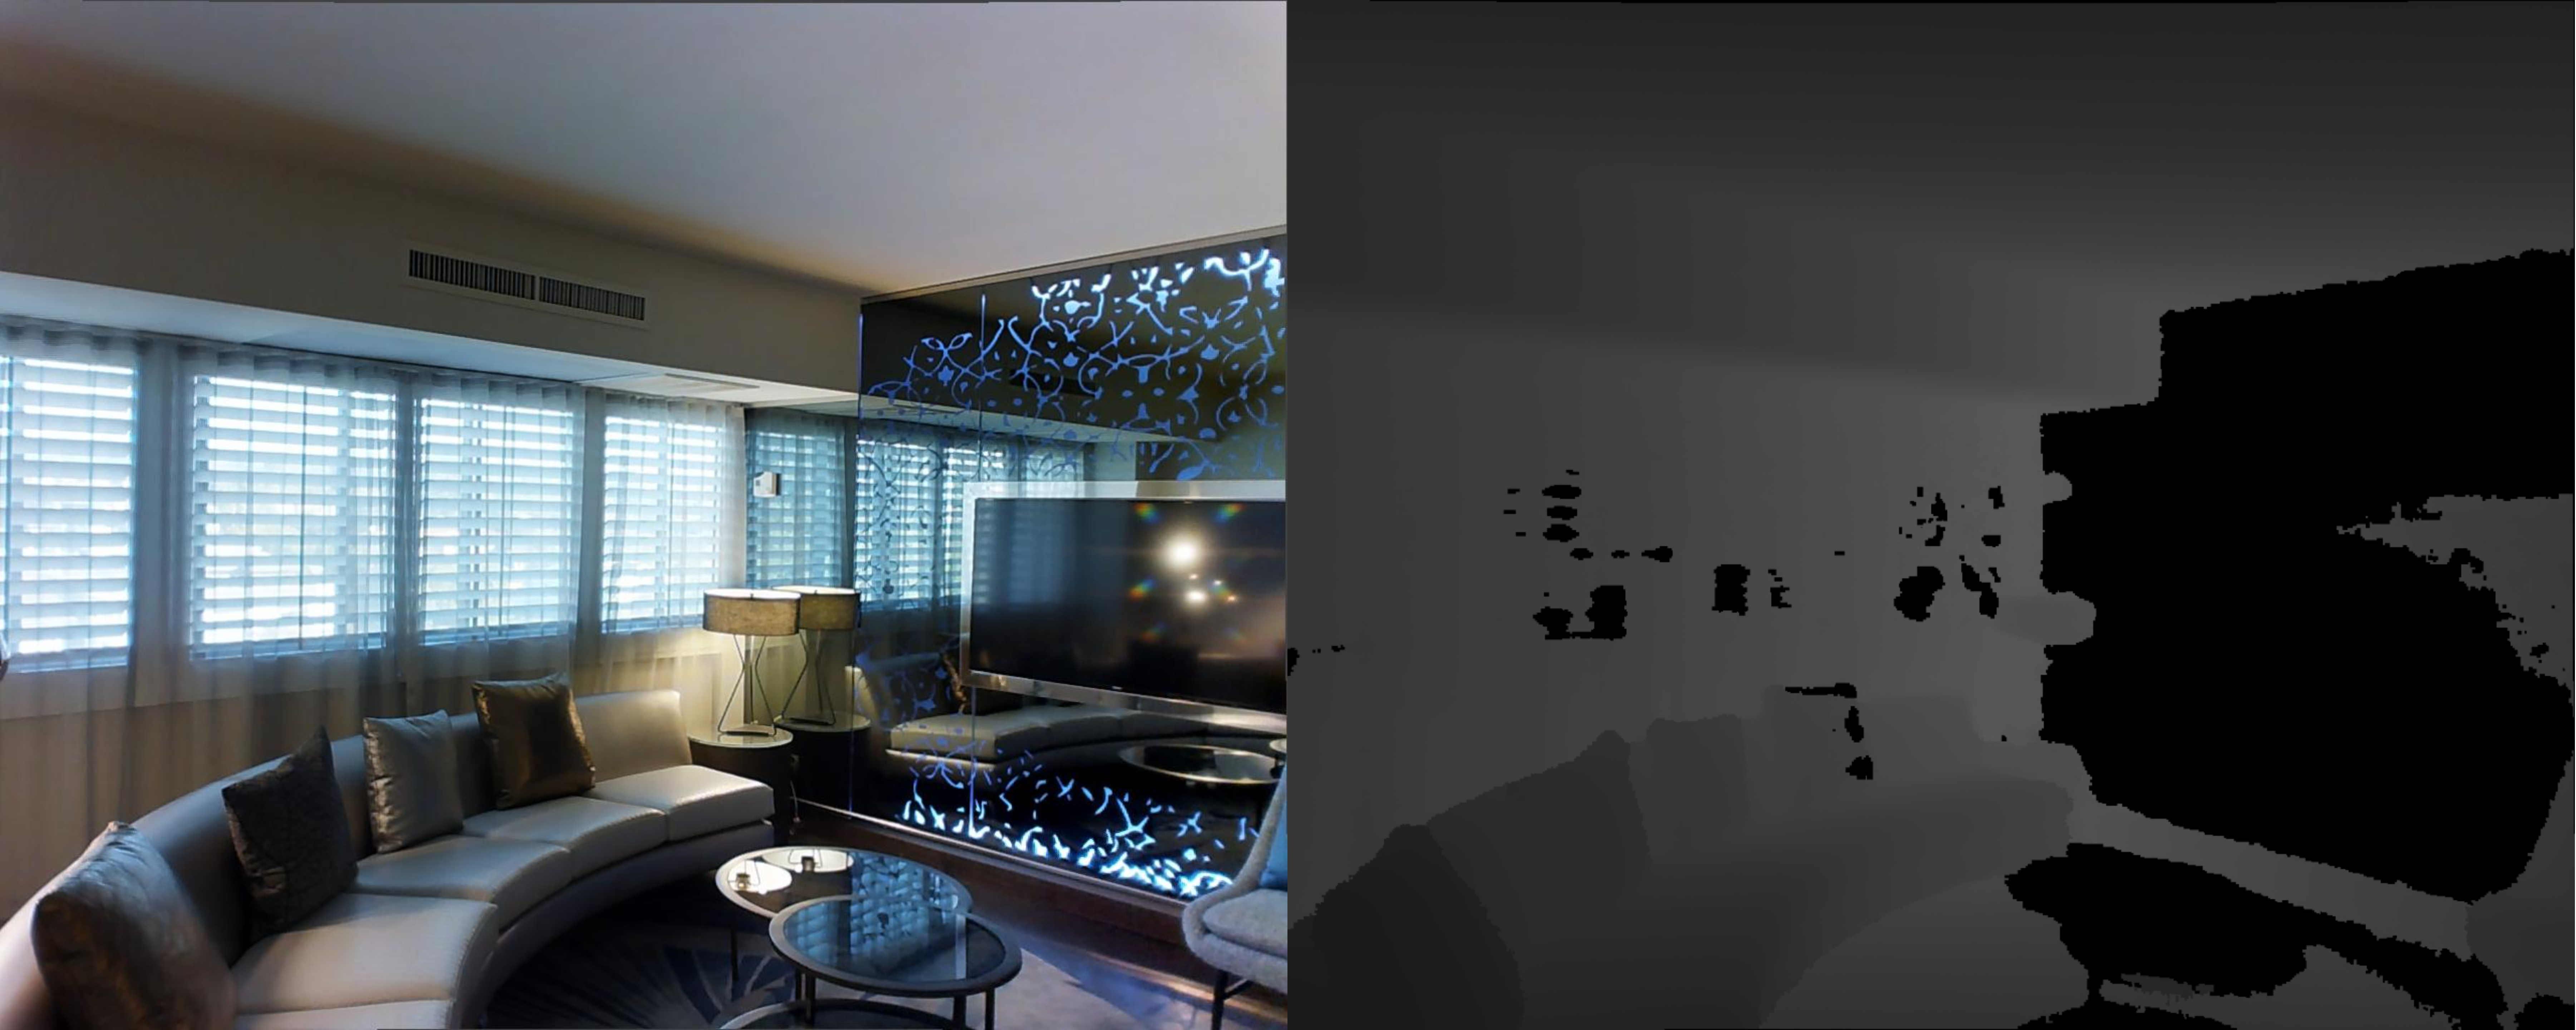
\includegraphics[width=\textwidth]{fig/depth_problema.png}
%     \caption{Exemplo de imagem RGB com mapa de profundidade apresentando leituras inválidas.}
%     \label{errdepth}
% \end{figure}

%problemas 27, 80, 98

Garantir a correta representação dos mapas em escala de pixel é de considerável importância para as tarefas que dependem de profundidade e que requerem um alto grau de segurança e confiabilidade dos dados, como veículos autônomos ou navegação de drones. A tecnologia LiDAR é a alternativa com implementação mais confiável entre as que foram citadas, no entanto, ressalta-se que nem o LiDAR e nem câmeras RGB-D convencionais produzem mapas completos e densos. No caso do LiDAR, são produzidos mapas esparsos (approx. 95\% de esparsidade) e no caso de câmeras RGB-D ou câmeras ToF são produzidos mapas com partes faltantes em determinadas superfícies ou bordas \cite{hu2012robust}. 




% Neste cenário, tecnologias de aquisição e melhoramento dos dados foram amplamente pesquisadas pela ciência nos últimos anos. Recentemente foram exploradas técnicas que não dependem de sensores de profundidade, ou seja, que inferem a informação de profundidade a partir de uma única imagem RGB capturada a partir de uma câmera comum, essa abordagem é conhecida como \textit{Monocular Depth Estimation} (MDE). No entanto, métodos baseados em características puramente visuais   \cite{szeliski2022computer} \cite{hu2022deep}. 



Considerando as limitações impostas por métodos ativos de aquisição de profundidade, surge a possibilidade de inferir um mapa de profundidade denso e completo de uma cena a partir de uma ou mais imagens RGB, processo conhecido como estimação de profundidade (\textit{Depth Estimation - DE}) \cite{rajapaksha2024deep}. Quando duas imagens de câmeras diferentes são utilizadas para obter-se a informação de profundidade, denomina-se \textit{Stereo Matching (SM)}. No entanto, métodos baseados em imagens \textit{stereo} requerem processos complexos de calibração e alinhamento \cite{dong2022towards}.


O problema da estimação monocular de profundidade (\textit{Monocular Depth Estimation - MDE}) tem por objetivo inferir o mapa de profundidade através de uma única imagem RGB. Esse problema é considerado mal-posto devido à ausência de informação geométrica na projeção da cena 3D para a imagem 2D. No entanto, os avanços nas tecnologias de \textit{Deep Learning - DL} e visão computacional tornaram factível e conveniente o uso de MDE para estimar mapas de profundidade densos e completos \cite{spencer2024third} \cite{rajapaksha2024deep}. 

Ao longo dos anos, houveram diversas pesquisas científicas abordando o tema de estimação monocular de profundidade utilizando toda a miríade de técnicas e metodologias dentro do universo do aprendizado profundo, empregando desde redes neurais convolucionais \cite{kopf2021robust}, estruturas \textit{encoder-decoder} \cite{godard2019digging}, mistura de bases de dados em grande escala em modos diferentes \cite{lasinger2019towards}, transformadores de visão \cite{birkl2023midas}, modelos de difusão \cite{ke2024repurposing}, e treinamento utilizando dados reais pseudo-rotulados em larga escala \cite{yang2024depth}. 

Neste cenário, este trabalho propõe uma análise comparativa entre os diversos modelos de estimação monocular de profundidade relativa baseados em aprendizado profundo através da abordagem quantitativa, utilizando métricas e \textit{benchmarks} presentes na literatura, abordagem qualitativa e através de uma aplicação. 



\section{Motivação e Justificativa} 

Os recentes avanços na área de MDE propiciaram a aquisição de informação de profundidade de maneira mais precisa e rápida, dessa forma, também favorecem indiretamente as aplicações que dependem desse tipo de dado, como reconstrução 3D, navegação e veículos autônomos. Além disso, devido à facilidade de implementação dessas técnicas, também podemos citar melhoramentos em aplicações mais modernas como conteúdo gerado por Inteligência Artificial \cite{yang2024depth}.


Reconstruir estruturas 3D a partir de imagens e informação geométrica prévia é um dos tópicos amplamente investigados pela ciência nos últimos anos \cite{zhao2020monocular}. A técnica \textit{Simultaneous Localization and Mapping} (SLAM) consiste planejar e controlar os movimentos de um robô por meio da construção de um mapa espacial do ambiente ao seu redor e obter a sua localização relativa, relacionando a área da visão computacional e a robótica através reconstrução de ambientes 3D e sensores de imagem \cite{placed2023survey} \cite{stachniss2016simultaneous}. Métodos de SLAM que objetivam a fusão de característica de mapas de profundidade obtidos através de sensores em movimento tiveram um aumento de popularidade em tempos recentes, visto que podem ser empregados para navegação e mapeamento de diversos tipos de dispositivos autônomos, como drones e robôs, além das aplicações em realidade aumentada e computação gráfica \cite{tateno2017cnn}.


Detectores de objetos com imagens tem sido aplicados em diversas áreas, como veículos autônomos e visão robótica, em que os sistemas necessitam estimar a localização de pedestres, veículos ou outros obstáculos. Devido à ausência informação de profundidade em imagens 2D, algumas aplicações exigem que a detecção seja feita no espaço tridimensional. O problema da detecção 3D consiste em estimar os vértices das caixas tridimensionais que contenham determinados objetos \cite{hu2022detection}. Uma das formas de adquirir a informação de profundidade necessária é através de LiDAR, entretanto, segundo \citeonline{wu2022sparse}, métodos de detecção 3D baseados somente em informação de LiDAR sofrem com a esparsidade dos dados, além do alto custo financeiro do equipamento. De acordo com \citeonline{ding2020learning} uma alternativa mais desejável é o uso de câmeras monoculares. Mapas de profundidade podem são empregados de duas formas: Transformando os mapas em representação pseudo-LiDAR, ou em sistemas multi-modais em conjunto com a informação RGB. A performance dos métodos de detecção 3D que utilizam informação de profundidade dependem da qualidade e densidade dos mesmos, portanto, as novas tecnologias de estimação monocular profundidade podem contribuir significativamente para este fim.






Segundo \citeonline{khan2020deep}, é evidente o potencial da estimação monocular para problemas de aplicações que envolvam informação de profundidade. Para que as diversas aplicações apresentadas possam funcionar de forma eficaz, é necessário garantir a correta representação dos mapas que são utilizados como entrada dos sistemas. Dado os recentes avanços nos modelos de MDE, tornou-se possível gerar mapas de profundidade de alta qualidade, com fineza de detalhes e de forma rápida, o que cobre as desvantagens de outros tipos de aquisição. 

Neste cenário, faz-se necessária a avaliação dos diversos modelos e técnicas de estimação monocular de profundidade do estado da arte, analisando tanto a sua capacidade de gerar mapas densos e precisos quanto à sua empregabilidade em aplicações práticas que envolvam informação de profundidade, que é a proposta do presente trabalho.

 
\section{Objetivos}


\subsection{Objetivo Geral}
Este trabalho possui como objetivo geral a análise comparativa de estimadores monoculares de profundidade robustos capazes de produzir informação de profundidade de alta qualidade para imagens sob quaisquer circunstâncias.

\subsection{Objetivos Específicos}

\begin{itemize}
    \item Estudo e escolha dos datasets que contenham imagens apropriadas para teste.
    \item Estudo de modelos de estimação monocular de profundidade relativa do estado da arte.
    \item Análise e escolha entre os modelos estudados para implementação e testes.
    \item Avaliação de desempenho perante métricas utilizadas na literatura para comparação entre os modelos no espaço relativo e métrico.
    \item Implementação de método de pós-processamento para transferência do domínio relativo para métrico baseado em transformação de intensidade.
    \item Avaliação qualitativa dos resultados.
    \item Implementação e avaliação de aplicação com os mapas de profundidade gerados a partir dos estimadores do estado da arte.
    
\end{itemize}


    \chapter{Trabalhos Relacionados}


No passado, a tarefa de Estimação Monocular de Profundidade não era abordada de forma direta. Um exemplo deste cenário é o trabalho de \citeonline{hoiem2005automatic}, em que o objetivo é reconstruir uma cena 3D em um ambiente virtual através de uma única imagem RGB. Apesar da finalidade não ser a construção de um mapa de profundidade, a reconstrução 3D de uma cena é diretamente ligada à informação de profundidade, portanto, esse trabalho é creditado em revisões bibliográficas do tema \cite{mertan2022single}. É considerado que um ambiente externo consiste de elementos fixos, o céu, um plano de chão e objetos verticais saindo deste plano. É realizada uma classificação de superpixels nas classes através de características pré-selecionadas manualmente, e os objetos são colocados em 3D através das mesmas.


Ainda nos primórdios da MDE, um dos primeiros trabalhos a se propor a estimar um mapa de profundidade métrico de uma única imagem RGB é o de \citeonline{saxena2005learning}. Filtros manualmente projetados são aplicados em pequenos pedaços de uma imagem de entrada para extrair características. Para cada parte, um valor de distância é estimado. Os filtros são então aplicados em múltiplas escalas para levar em consideração as pistas visuais globais e de partes adjacentes. Pesos maiores são atribuidos às características dos pedaços que ficam nas mesmas colunas, baseado na premissa de que as estruturas dos objetos observados são em sua maioria, verticais. Além disso, um modelo baseado em Campos Aleatórios de Markov (\textit{Markov Random Field} - MRF) é treinado de maneira supervisionada para estimar a profundidade a partir das características.


Algum tempo depois, outro trabalho publicado por \citeonline{saxena2008make3d}, adicionou um pressuposto pertinente ao estado da arte de MDE, que uma cena consiste de várias pequenas superfícies planas e a orientação e localização 3D dessa superfície podem ser utilizadas para calcular sua profundidade. Esse pressuposto é utilizado até hoje em motores gráficos que criam modelos de objetos complexos através de malhas triangulares. Novamente, é utilizado um modelo baseado em MRF treinado de maneira supervisionada. As características são obtidas através de filtros manualmente projetados e a contextualização global é considerada através de superpixels adjacentes.


Considerando o desenvolvimento do aprendizado profundo à época, \citeonline{eigen2014depth} introduziu o uso de redes neurais convolucionais para a tarefa de MDE, superando as técnicas anteriores. O problema foi formulado como um método de regressão com aprendizado supervisionado de um conjunto de duas redes neurais. A primeira é responsável por uma estimação grosseira do mapa de profundidade. Sendo composta por camadas convolucionais totalmente conectadas, possui a imagem toda como campo receptivo, utilizando melhor o contexto global, a custo de um grande custo computacional. A segunda rede neural é totalmente convolucional e possui como entrada o mapa da rede anterior, e tem como finalidade o ajuste fino do mapa de profundidade, operando através de filtros locais. Além disso foi utilizada uma função de perda com invariância em escala no espaço logarítmico.

A pesquisa realizada por \citeonline{ranftl2020towards} possui como principal contribuição o desenvolvimento de protocolos de mesclagem de conjuntos de dados de profundidade mesmo que suas anotações não sejam compatíveis. O núcleo dessa abordagem consiste em uma função que é invariante em escala e alcance em um processo de aprendizado multi-objetivo combinando dados de diferentes fontes. A arquitetura da rede consiste em uma estrutura baseada em ResNet em multi escala. Outra contribuição foi o emprego de filmes 3D para composição da base de dados de treinamento em larga escala, apesar de não apresentar anotação de profundidade, foi utilizado \textit{stereo matching} para obtenção do \textit{groundtruth}. 

Em \cite{ke2024repurposing} foi apresentado um protocolo de \textit{fine tuning} de modelos de difusão latente pré-treinados para estimação relativa de profundidade sob qualquer circunstância. O protocolo, chamado de Marigold, contribui com o estado da arte sendo um dos trabalhos que investigou o uso de bases de dados de imagens sintéticas para treinamento, dado que estas não estariam propensas a erros de captura. Utilizou-se um modelo de difusão estável pré-treinado, e o ajuste do modelo é realizado utilizando uma função objetivo calculada no espaço latente entre a saída da U-Net e o ruído inicial. Outra contribuição do trabalho foi a aplicação de ruído rectificado em multi resolução no processo de difusão. 

    


\chapter{Fundamentação Teórica}

\section{Processamento Digital de Imagens}

\section{Deep Learning}

\section{Informação de profundidade}

\section{Modelos de estimação de profundidade}

    
\chapter{Materiais e Métodos}

Para avaliar os modelos de estimação de profundidade, será utilizado o protocolo de \textit{zero-shot cross-dataset transfer}, i.e. realizar os testes e métricas em bases de dados que não compuseram os conjuntos de treinamentos dos modelos analisados. A performance em \textit{cross-dataset} é considerada uma aproximação mais fiel da performance em mundo real em uma aplicação, pois os conjuntos de testes relativos aos conjuntos utilizados no treinamento podem refletir os mesmos vieses e situações \cite{ranftl2020towards}.


\section{Datasets}

Bases de dados para treinamento ou teste de algoritmos de estimação de profundidade consistem em imagens RGB de uma cena e sua anotação correspondente em profundidade. Ao longo do tempo, diversos \textit{datasets} foram propostos para este fim com variações em formatos de anotações, tipos de cena (interior ou exterior), métodos de captura, qualidade, resolução e tamanho.

% \textcolor{red}{colocar citações que tem na seção 3 do midas 1}.

Geralmente são empregados sensores e outras tecnologias como \textit{Stereo Matching} e \textit{Structure from Motion} para criar os \textit{datasets} de profundidade, porém, são abordagens muito complexas, custosas, ou inviáveis em algumas situações particulares, por exemplo, obter mapas de profundidades densos a partir de veículos em movimento  \cite{yang2024depthv1}.
Cada \textit{dataset} possui suas próprias características, problemas e viéses. Dados com informação de profundidade e em alta qualidade são complexos de adquirir, sendo que os melhores conjuntos são utilizados no treinamento dos modelos presentes na literatura \cite{ranftl2020towards}. 



Dessa forma, para escolha das bases de dados a serem utilizadas para teste, temos os critérios: i) não ter composto o conjunto de treinamento dos modelos escolhidos para comparação, ii) conter dados válidos para avaliação considerando anotações precisas de profundidade, ou caso sejam esparsas, possuam máscara para indicar os pixels válidos, iii) ser uma base de dados conceituada na literatura. Os \textit{datasets} escolhidos e suas características podem ser visualizados na Tabela \ref{tabdata}.

% PESQUISA ANTIGA -------------------------------------------------------------------
% O presente trabalho exige um tipo de base de dados pouco encontrado na literatura, trios de imagem RGB, mapa de profundidade com erros e um outro mapa de profundidade denso e completo. De acordo com \cite{zhang2018deep}, uma das maneiras de se obter esses dados seria capturar imagens com uma câmera RGB-D de baixo custo e alinha-las com outra captura simultânea de um sensor mais preciso, porém essa abordagem é muito custosa, além de que não há disponibilidade de grandes conjuntos para treinamento.

% O presente projeto pretende utilizar como base de dados principal o \textbf{Hypersim}. Um \textit{dataset} para compreensão de cenas baseado em cenas sintéticas fotorrealistas. Contendo 77.400 imagens de 461 cenas \textit{indoor} com pares de RGB e mapas de profundidade calculado deterministicamente, além de outras informações como normais de superfície, rótulos de segmentação e detecção de objetos e entre outros \cite{roberts2021hypersim}.

% Please add the following required packages to your document preamble:
% \usepackage{graphicx}
\begin{table}[h]
    \centering
    \caption{Características dos datasets utilizados no trabalho}
    \label{tabdata}
    \resizebox{\textwidth}{!}{%
    \begin{tabular}{ccccccc}
    \hline
    \textbf{Dataset} & \textbf{Sensor} & \textbf{Anotação} & \textbf{Tipo} & \textbf{Cenário} & \textbf{Num. Imagens} & \textbf{Resolução} \\ \hline
    KITTI  & LiDAR         & Esparsa & Real      & Outdoor        & 44 K   & 1024 $\times$ 320  \\
    Nyu-V2 & Kinect V1     & Densa   & Real      & Indoor         & 1449   & 640 $\times$ 480   \\
    DIODE  & Laser Scanner & Densa   & Real      & Indoor/Outdoor & 25,5 K & 768 $\times$ 1024  \\
    SINTEL & -             & Densa   & Sintético & Indoor/Outdoor & 1064   & 1024 $\times$ 436  \\
    ETH3D  & Laser Scanner & Densa   & Real      & Indoor/Outdoor & 454    & 6048 $\times$ 4032 \\ \hline
    \end{tabular}%
    }
    \end{table}


\subsection{NYUv2}


%% refazer o texto

O \textit{dataset} NYUv2 é um dos mais utilizados em tarefas de visão computacional que envolvam estimação de profundidade, segmentação de cenas e reconecimento de objetos. Possui 1449 pares de imagens RGB e mapas de profundidade densos em diversas cenas \textit{indoor} divididos em 795 para treinamento e 654 para teste \cite{silberman2012indoor}. A resolução das imagens é de 640 $\times$ 480 pixels. O equipamento de aquisição foi o equipamento Microsoft Kinect que utiliza a técnica de emissão de luz estruturada, que produz resultados precisos de informação de profundidade. Além dos pares RGB-D, também é disponibilizado os dados de leitura dos sensores puros em que é possível encontrar aproximadamente 70\% de pixels com informação válida de profundidade, no entanto, as imagens finais foram processadas utilizando um método de correção, resultando em um mapa denso, como observado na Figura \ref{exnyuv2}. Entre as cenas observadas no \textit{dataset}, podemos citar quartos, cozinhas, sala de aula, banheiro e etc. Além das informações de profundidade, a base de dados provém rótulos de segmentação de objetos e relações de suporte entre eles \cite{lahiri2024deep}.

\begin{figure}[h]
    \centering
    \includegraphics[width=\textwidth]{fig/example_nyu.png}
    \caption{Exemplo do dataset NYU Depth v2}
    \label{exnyuv2}
\end{figure}

\subsection{KITTI}



\subsection{SINTEL}

\subsection{ETH3D}

O ETH3D é uma base de dados geralmente utilizada para reconstrução em vistas múltiplas e \textit{stereo matching}. Contém dados de treinamento com imagens RGB \textit{multiview}, capturadas com câmeras DSLR e \textit{ground truth} de profundidade capturado utilizando um escâner a laser Faro Focus X 330. Oferece três versões de imagens de profundidade, uma correspondente à leitura bruta do sensor (\textit{raw}), outra com \textit{outliers} removidos por trabalho manual e uma ferramenta automática (\textit{clean}) e uma com \textit{outliers} e pontos observados por uma única imagem RGB removidos. A partição de teste não contém \textit{groundtruth}. A base de dados é associada à um desafio aberto ao público. Inclui cenas tanto internas quanto externas, oferecendo um protocolo de avaliação bem variado \cite{lahiri2024deep} \cite{schops2019bad}. 

\subsection{DIODE}

O \textit{dataset} DIODE (\textit{Dense Indoor and Outdoor Depth Dataset}), é uma base de dados para estimação monocular de profundidade e consiste em 8574+25 imagens de ambientes internos e 16.884+446 de ambientes externos para treinamento e teste. Possui resolução de 768 $\times$ 1024 com faixa de distâncias entre 50m e 300m para os ambientes internos e externos respectivamente. O equipamento de aquisição é o escâner a laser Faro Focus S350. Alguns exemplos do \textit{dataset} podem ser visualizados na Figura \ref{exdiode}.

\begin{figure}[h]
    \centering
    \includegraphics[width=\textwidth]{fig/example_diode.png}
    \caption{Exemplo do dataset DIODE}
    \label{exdiode}
\end{figure}

\section{Modelos Escolhidos}

\section{Protocolo de Avaliação}

\section{Método de Transformação de Intensidades (pós-processamento)}

Um mapa de profundidade inferido por um método de estimação de profundidade possui a característica de ser denso, pois todos os pixels possuem um valor predito associado, preciso, bem detalhado, de acordo com os últimos trabalhos do estado da arte porém é relativo, i.e. o valor de cada pixel é apenas correlacionado com a medição de distância real por um fator desconhecido. Já um mapa de profundidade adquirido com um sensor físico consegue representar as grandezas de forma métrica (em metros, centímetros ou até milimétros), mas pode ter características negativas associadas a depender do dispositivo de aquisição, podendo conter áreas falhas que não possuem medição associada, ou um elevado grau de esparsidade. O método de transformação de intensidades para transferência de domínio almeja como resultado uma imagem de profundidade que possuam as características positivas dos dois casos anteriormente citados. 

O método proposto por este trabalho consiste em uma transformação de intensidades que é projetada para cada imagem de um conjunto de dados utilizando pontos correspondentes em ambas e associando uma transformação linear para cada ponto, como visualizado na Figura \ref{posproc}. 


\begin{figure}[h]
    \centering
    \includegraphics[width=\textwidth]{fig/diagram_normalization_white.png}
    \caption{Diagrama do método de transferência de domínio}
    \label{posproc}
\end{figure}

O método proposto diferencia-se do tradicional baseado em fator de escala e deslocamento por mínimos quadrados pois é associada uma função linear para cada região na quantização da imagem, o que propicia uma correção adaptada para cada proporção de distância. Ressalta-se que o método não será utilizado no protocolo de avaliação dos modelos de estimação de profundidade.

será realizada a comparação do resultado da técnica de pós-processamento e o resultado de estimadores métricos de profundidade com os conjuntos de dados que possuem leituras métricas de sensores.


\section{Análise com Aplicação}

Para avaliar os mapas de profundidade gerado pelos modelos do estado da arte, será utilizada também uma ou mais aplicações práticas. O processo de escolha da aplicação a ser implementada e avaliada passa por três principais critérios, entre eles: 

\begin{itemize}
    \item Empregar diretamente como entrada do sistema um mapa de profundidade denso.
    \item Possuir código de testes público.
    \item Ter o seu desempenho mensurável através de métricas. 
\end{itemize}





\section{Considerações Metodológicas}


    
\chapter{Resultados e Discussões}

\section{Resultados Preliminares}


\section{Resultados Esperados}






    \chapter{Cronograma}

Este capítulo visa expor as atividades já realizadas e futuras considerando os prazos estipulados para finalização da pesquisa científica e defesa de dissertação. A tabela \ref{cron23} mostra as atividades realizadas no ano de 2023 e a Tabela \ref{cron24} para o ano 2024 e Janeiro de 2025. 

% Please add the following required packages to your document preamble:
% \usepackage{graphicx}
\begin{table}[H]
    \centering
    \caption{Cronograma com as atividades realizadas para o desenvolvimento da pesquisa do ano de 2023}
    \label{cron23}
    \resizebox{\textwidth}{!}{%
    \begin{tabular}{|c|c|c|c|c|c|c|c|c|c|c|c|c|}
    \hline
    ATIVIDADES                                                                         & JAN & FEV & MAR & ABR & MAI & JUN & JUL & AGO & SET & OUT & NOV & DEZ \\ \hline
    \begin{tabular}[c]{@{}c@{}}Alinhamento do\\ projeto de pesquisa\end{tabular}       & X   & X   & X   & X   & X   & X   &     &     &     &     &     &     \\ \hline
    Revisão Bibliográfica                                                              &     &     &     &     &     & X   & X   & X   & X   & X   & X   & X   \\ \hline
    \begin{tabular}[c]{@{}c@{}}Aquisição e Análise de\\ Datasets\end{tabular}          &     &     &     &     &     &     & X   & X   &     &     &     &     \\ \hline
    \begin{tabular}[c]{@{}c@{}}Implementação de \\ modelos de segmentação\end{tabular} &     &     &     &     &     &     &     & X   & X   & X   &     &     \\ \hline
    Testes dos modelos                                                                 &     &     &     &     &     &     &     &     &     & X   & X   &     \\ \hline
    \begin{tabular}[c]{@{}c@{}}Realinhamento de pesquisa:\\ Aplicações de \\ mapas de profundidade\end{tabular} &  &  &  &  &  &  &  &  &  &  &  & X \\ \hline
    \end{tabular}%
    }
    \end{table}




% Please add the following required packages to your document preamble:
% \usepackage{graphicx}
\begin{table}[ht]
    \centering
    \caption{Cronograma com as atividades realizadas e pretendidas para o desenvolvimento da pesquisa do ano de 2024 e Janeiro de 2025.}
    \label{cron24}
    \resizebox{\textwidth}{!}{%
    \begin{tabular}{|c|c|c|c|c|c|c|c|c|c|c|c|c|c|}
    \hline
    ATIVIDADES                                                                     & JAN & FEV & MAR & ABR & MAI & JUN & JUL & AGO & SET & OUT & NOV & DEZ & JAN \\ \hline
    \begin{tabular}[c]{@{}c@{}}Revisão \\ Bibliográfica\end{tabular}               & X   & X   & X   & X   & X   & X   & X   & X   & X   & X   & X   & X   & X   \\ \hline
    \begin{tabular}[c]{@{}c@{}}Realinhamento de pesquisa:\\ Correção de mapas \\ de profundidade\end{tabular}       &  & X &   &   &   &   &   &  &   &  &  &  &  \\ \hline
    \begin{tabular}[c]{@{}c@{}}Estudo de técnicas de\\  correção de profundidade\end{tabular}                       &  & X & X & X &   &   &   &  &   &  &  &  &  \\ \hline
    \begin{tabular}[c]{@{}c@{}}Análise de\\ datasets de correção \\ de profundidade\end{tabular}                    &  &   & X & X & X &   &   &  &   &  &  &  &  \\ \hline
    \begin{tabular}[c]{@{}c@{}}Implementação de técnicas \\ de correção   \\  de profundidade\end{tabular}          &  &   &   & X & X & X &   &  &   &  &  &  &  \\ \hline
    \begin{tabular}[c]{@{}c@{}}Realinhamento de pesquisa: \\ Análise de estimadores \\ de profundidade\end{tabular} &  &   &   &   &   &   & X &  &   &  &  &  &  \\ \hline
    \begin{tabular}[c]{@{}c@{}}Aquisição e análise \\ de datasets\end{tabular}     &     &     &     &     &     &     & X   &     &     &     &     &     &     \\ \hline
    Execução de experimentos                                                       &     &     &     &     &     &     & X   & X   &     &     &     &     &     \\ \hline
    \begin{tabular}[c]{@{}c@{}}Análise comparativa \\ dos estimadores\end{tabular} &     &     &     &     &     &     & X   & X   &     &     &     &     &     \\ \hline
    Exame de qualificação                                                          &     &     &     &     &     &     &     & X   & X   &     &     &     &     \\ \hline
    \begin{tabular}[c]{@{}c@{}}Implementação de \\ Transformação de intensidade\end{tabular}                        &  &   &   &   &   &   &   &  & X &  &  &  &  \\ \hline
    Implementação de aplicação                                                     &     &     &     &     &     &     &     &     & X   &     &     &     &     \\ \hline
    \begin{tabular}[c]{@{}c@{}}Análise dos resultados \\ da aplicação\end{tabular} &     &     &     &     &     &     &     &     &     & X   &     &     &     \\ \hline
    Escrita de texto de dissertação                                                &     &     &     &     &     &     &     &     &     &     & X   & X   & X   \\ \hline
    \begin{tabular}[c]{@{}c@{}}Revisão final/\\ Defesa da Pesquisa\end{tabular}    &     &     &     &     &     &     &     &     &     &     &     &     & X   \\ \hline
    \end{tabular}%
    }
    \end{table}

% --- -----------------------------------------------------------------
% --- Referencias Bibliograficas. (Obrigatorio)
% --- -----------------------------------------------------------------
    \cleardoublepage
%    \bibliographystyle{acm-2} % abbrv - abnt-num
	%\bibliographystyle{plainnat}
    \bibliography{bibliografia} % arquivo fonte com a bibilografia

% --- -----------------------------------------------------------------
% --- Apendice.(Opcional)
% --- -----------------------------------------------------------------
    \cleardoublepage
    \appendix
        \chapter{Apêndice A}
\label{appendixA}

...
    %     % \include{appendixB}
    %     % \include{appendixC}
    %     % \include{appendixD}
    %     % \include{appendixE}
    %     % \include{appendixF}
    %     % \include{appendixG}
    %     % \include{appendixH}
    %     % \include{appendixI}
    %     % \include{appendixJ}
    %     % \include{appendixK}
    %     %\include{appendixL}
    % \end{landscape}
\end{document}